\chapter{Regression}

Regression is a form of supervised machine learning with as goal to take continuous data and find the equation that best fits the data. This way you'll be able to forecast a specific value.

\section{Linear Regression}
The best fit function searched is just a linear line. See figure \ref{fig:linearregression} for an example.

\begin{figure}
\centering
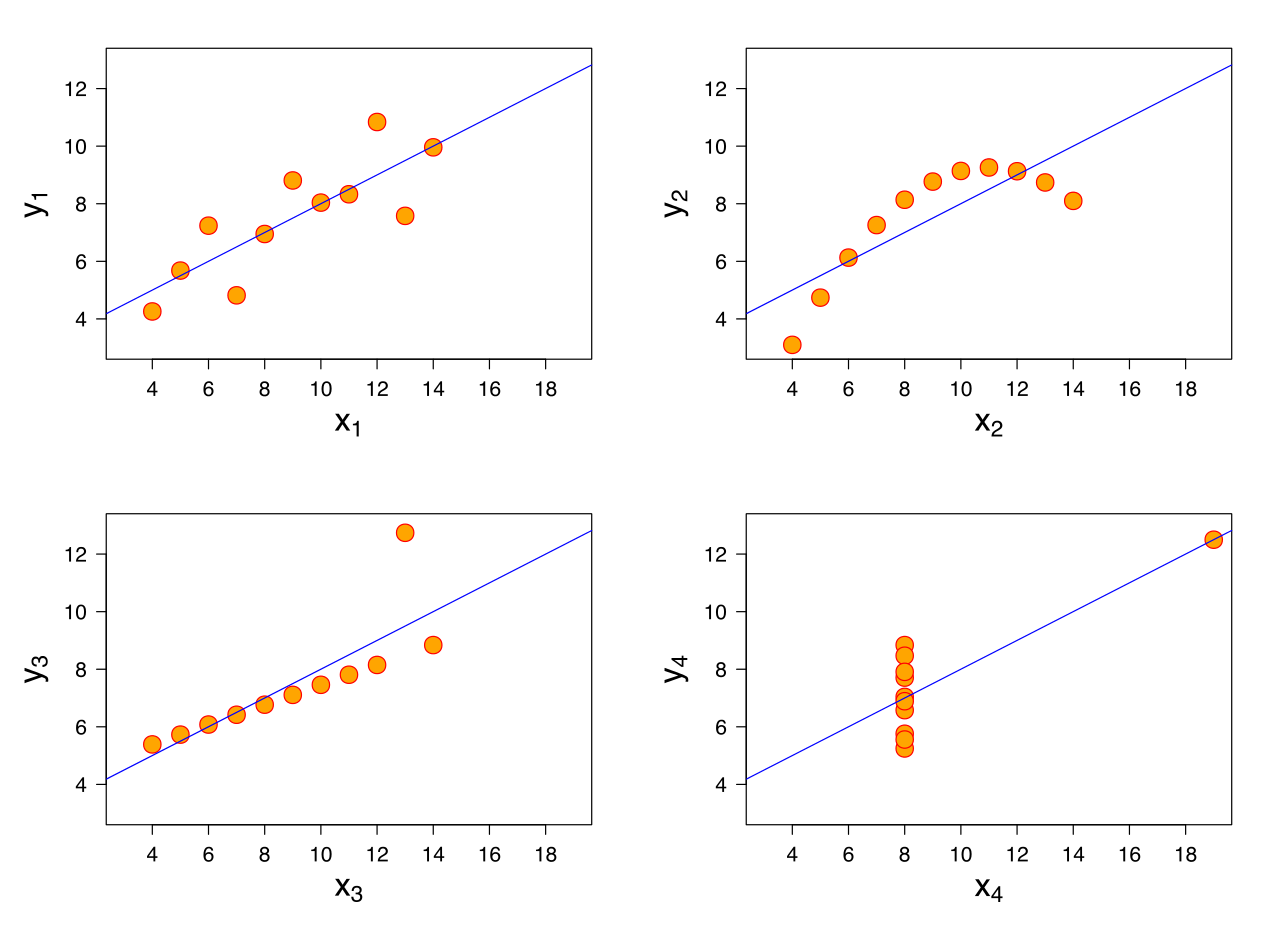
\includegraphics[width=1\textwidth]{images/linear_regression.png}
\caption{\label{fig:linearregression}Four examples of the function found by linear regression based on the given data points.}
\end{figure}
